\chapter{Experimental Methodology} 

Our initial goal was to implement a couple of algorithms as baseline for
experiments outside of the scope of this work. Ideally, those algorithms would
have also helped us finding any ``low-hanging fruits'' to properly start
tackling the game as a whole. In addition to implementing those algorithms, we
also designed a few automatic tests to check the validity of the game state
information in known maps.  

\section{Test Task}

\section{RL Algorithms}

At the start of the project we decided that by the end of it we would have had a
classic model-free RL algorithm to test an MDP-like setting and the newer DQN, a
deep reinforcement learning algorithm, to test learning policies purely from the
visual input. 

\subsection{Q-learning}

The choice of Q-learning as the test model-free algorithm was relatively
straightforward: Q-learning is one of the most popular and powerful model-free
RL algorithms, and it represents the foundation of many other reinforcement
learning algorithms. Given a standard MDP in the form of a tuple $(S, A, T, R)$
where $S$ is the state space, $A$ is the action space, $T(s, s')$ is the
transition probability distribution of moving from state $s$ to state $s'$, and
$R$ is the immediate reward received when moving from state $s$ to state $s'$,
Q-learning allows to iteratively find a policy that maximises the expected total
reward in a trial by learning from experience gained by some policy (as opposed
to on-policy reinforcement learning where the samples are  to the
policy being learnt).

In particular, the algorithms works by updating an action-value function $Q(s,
a)$ using an $\epsilon$-greedy policy to gain new samples. Given a learning rate
$\alpha$ and a discount factor $\gamma$,

\begin{equation}
  Q(s_t, a_t) = Q(s_t, a_t) + 
  \alpha \bigg[ r_{t+1} + \gamma \max_a Q(s_{t+1}, a_{t+1}) - Q(s_t, a_t) \bigg].
\label{eq:ql}
\end{equation}

The agent policy in the evaluation phase then becomes

\begin{equation}
  \pi(s, a) = \operatornamewithlimits{argmax}_a Q(s, a).
\label{eq:ql2}
\end{equation}

It has been proved that this policy converges to the optimal policy $\pi*$ given
enough samples from all state-action pairs. % TODO how?

The Q function can be represented as a table of values (a simple array) or can
be approximated using a function approximator, however a lot of literature has
highlighted difficulties in making Q-learning (and other model-free RL
algorithms) converge when the action-value function is approximated
\citep{Baird_1997}. In some cases researched managed to converge the algorithms,
but obtained significantly degraded policies \citep{bertsekas_1996_tetris,
  waver_and_baxter_1999, boyan_and_moore_1995}.

\subsubsection{Task dependent state representation}

Providing a state representation for quickly testing the whole system ended up
resulting in a far more challenging problem than initially estimated. To be able
to extensively test the symbolic game state data being sent by the client we
wanted to obtain a useful state representation without having to use a black-box
function approximator such as an artificial neural network. Using a neural
network would have made it very hard to do automatic testings. Moreover we
wanted to check and explore how difficult it would have been to use standard RL
techniques on StarCraft's large state space.

\begin{figure}[h]
    \centering
    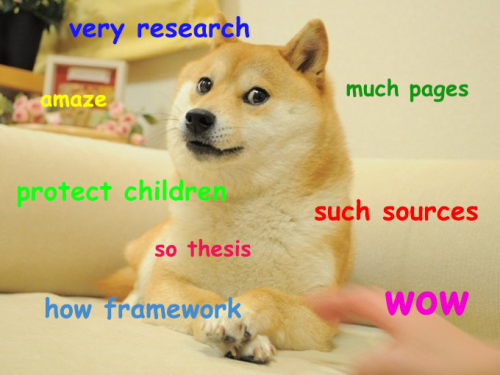
\includegraphics[width=0.9\textwidth]{placeholder}
    \caption{Example of a state in our test domain.}
    \label{fig:sample_state}
\end{figure}

Figure \ref{fig:sample_state} shows a sample of the game state data in our
domain. We can see that it is difficult to represent such a representation in an
array because the data increases with the number of units. To create a
representation that we can use in a tabular fashion we must approximate the
state in some way.

\begin{figure}[h]
    \centering
    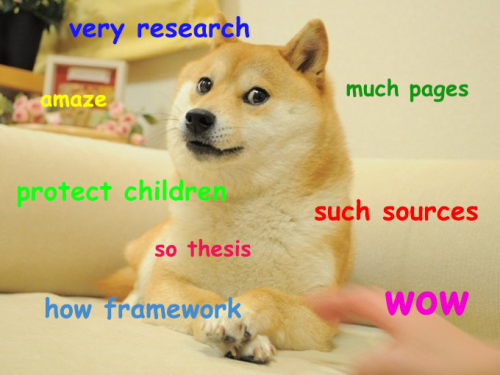
\includegraphics[width=0.9\textwidth]{placeholder}
    \caption{Discretisation of state based on units health points.}
    \label{fig:discrete_state}
\end{figure}

We chose to approximate the state by discretise a potential function
\citep{diebelthrun} based on the health points of in-game units relative to a
particular selected allied unit (Figure \ref{fig:discrete_state}). This was
achieved by taking a particular unit as reference, filtering out everything
lying outside of the visible pixel radius, splitting then the obtained space
into a variable amount of slices. The value of each slice was then calculated by
obtaining the sum of all health ``value'' assigned to each unit within a space.
Given slice $p$ and $U_p$ units, the slice value $SV(p)$ is computed as

\begin{equation}
  \begin{aligned}
    SV(p, \beta) = & 
    \begin{cases}
      \sum_{u \in U_p}{UV(u)} & \text{if } \sum_{u \in U_p}{UV(u)} < \beta \\
      \beta & otherwise\\
    \end{cases}, \\ \text{where } 
    UH(u) = &
    \begin{cases}
      1 & \text{if } \text{health}_u < 50\%\\
      2 & otherwise \\
    \end{cases} 
  \end{aligned}
\end{equation}

We created a pair of partitions for each class of unit representing allied units
and enemy units, and added to the top the value of the reference unit health,
ending up with a relatively large tensor as our index for our action-value
function (Figure \ref{fig:array_state}).

\begin{figure}[h]
    \centering
    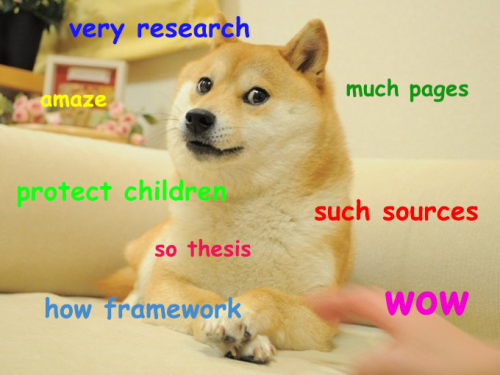
\includegraphics[width=0.9\textwidth]{placeholder}
    \caption{Mapping from slices to index tensor.}
    \label{fig:array_state}
\end{figure}

We could have also used a tile-coding
technique\citep{stone_sutton_keepaway} to increase the generality of our state
representation by stacking multiple partitions of the same space (but different
starting points), but we didn't have the time to finish its implementation.

This approximation is reasonable (as tests later confirmed) for our task, but it
would necessarily lend itself well to other scenarios. Our representation for
instance entirely lacks information about upgrades, bullets, visibility of the
map and state of the fog of war. It must be noted that with this representation
the problem becomes more complex than a standard MDP, as we are not using the
entirety of the available state information by filtering everything outside of
the image radius. We could have also used an observation window to solve the
partial observability problem, but we hypothesised that we would obtain a good
enough (but almost certainly suboptimal) policy in any case.

% TODO add missing sliding state windows.

\subsection{DQN}

\subsection{Multi-unit RL}


\section{Experimental Setup}
